\documentclass[a2paper]{article}

\usepackage{siunitx}
\usepackage{tikz}
\usetikzlibrary{arrows}
\usepackage{amsmath}
\usepackage{geometry}
% \usepackage{showframe}

\geometry{a2paper,margin=0.5in}
\pagestyle{empty}

\begin{document}
\thispagestyle{empty}

\begin{figure}[h!]
\begin{tikzpicture}
\node[anchor=south west,inner sep=0] at (0.2,-5.0) 
{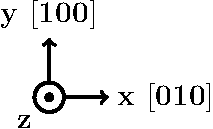
\includegraphics[width=0.30\textwidth]{arrows1}};
\node[anchor=south west,inner sep=0] at (0.2,-0.3) 
{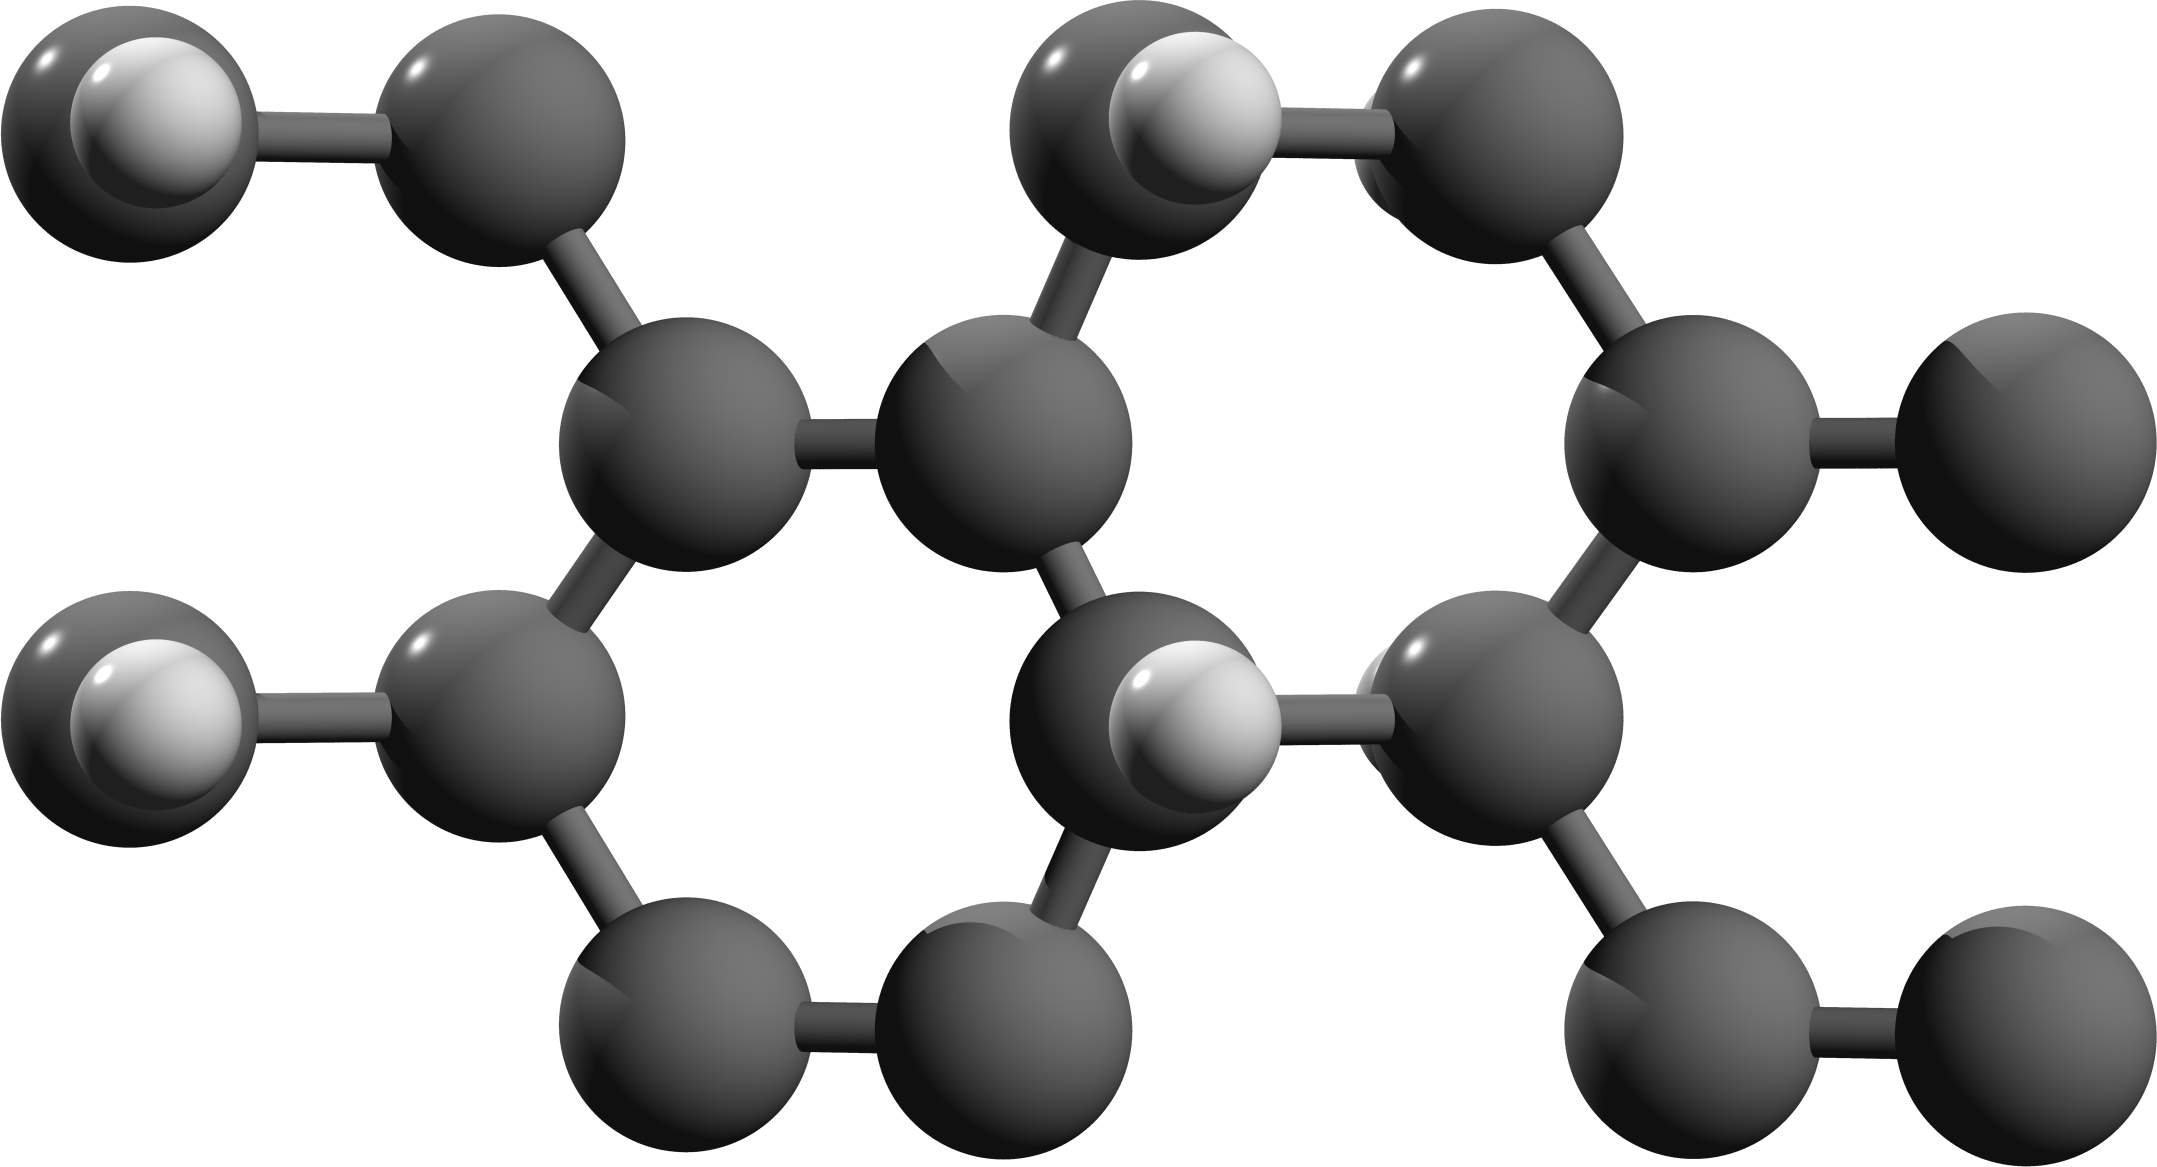
\includegraphics[width=\textwidth]{alt1}};
\draw [line width=2.00mm, red, -> ] (2.80,07.50) -- (2.80,19.00) 
node [right] {};
\draw [line width=2.00mm, red, -> ] (2.80,07.50) -- (22.00,07.50) 
node [right] {};
\draw [line width=2.00mm, red, dash pattern=on 10pt off 5pt] (22.00,07.50) --
(22.00,19.00) node [right] {};
\draw [line width=2.00mm, red, dash pattern=on 10pt off 5pt] (2.80,19.00) --
(22.00,19.00) node [right] {};

\draw [] ( -1.00, 11.00) node [right] {\scalebox{6.0}{C$_{1}$}};
\draw [] (  5.00, 11.00) node [right] {\scalebox{6.0}{C$_{2}$}};
\draw [] ( 13.00, -1.00) node [right] {\scalebox{6.0}{C$_{3}$}};
\draw [] ( 19.00, -1.00) node [right] {\scalebox{6.0}{C$_{4}$}};
\draw [line width=2.00mm, black, <- ] ( 3.50,  7.30) -- (  5.50,  5.00)
node [right] {\scalebox{6.0}{H$_{1}$}};

\node[anchor=south west,inner sep=0] at (0.2,-34.0) 
{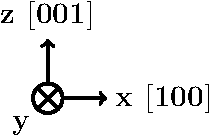
\includegraphics[width=0.30\textwidth]{arrows2}};
\node[anchor=south west,inner sep=0] at (0.2,-24.6) 
{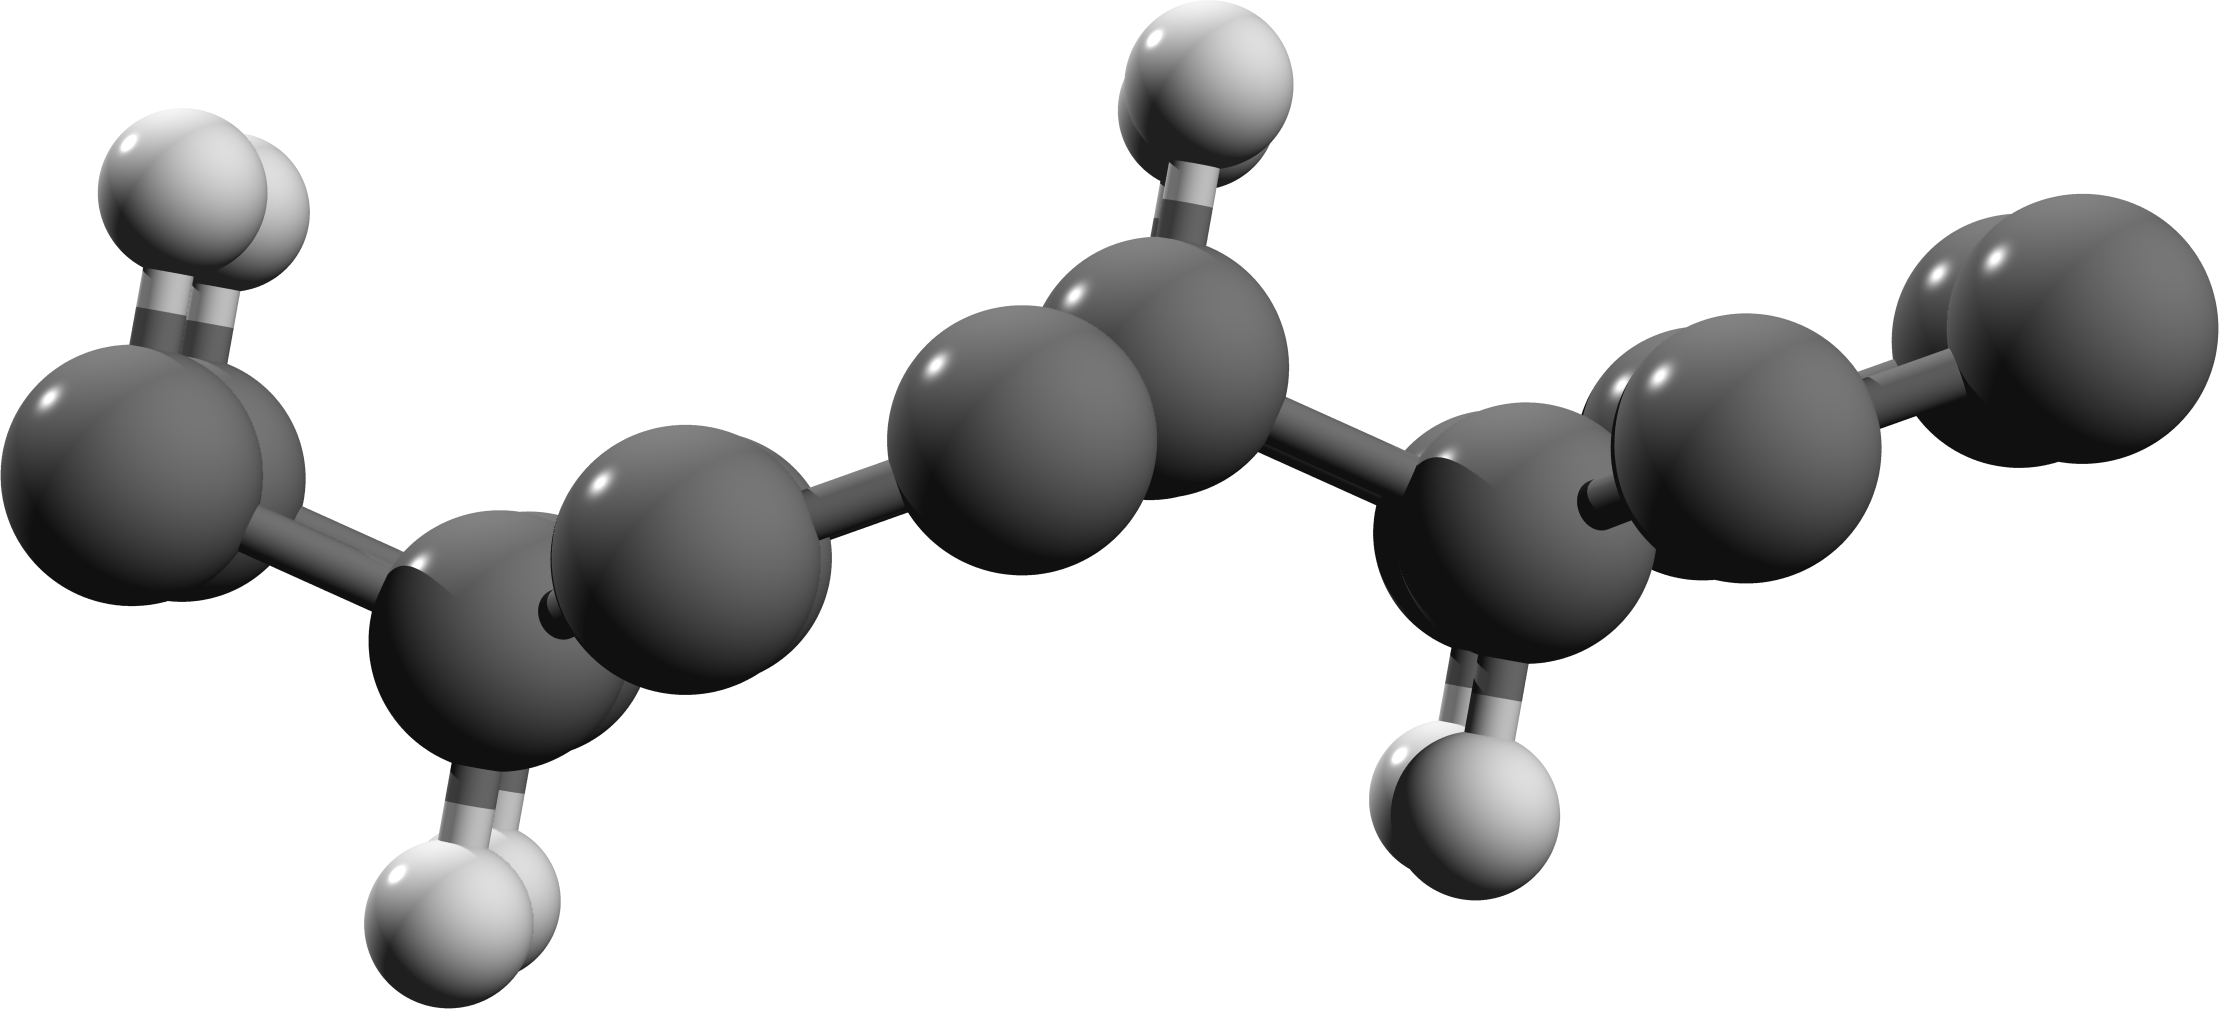
\includegraphics[width=\textwidth]{alt2}};

\draw [] ( -1.00, -10.50) node [right] {\scalebox{6.0}{H$_{1}$}};
\draw [] (  0.50, -19.50) node [right] {\scalebox{6.0}{C$_{1}$}};
\draw [] (  4.50, -20.50) node [right] {\scalebox{6.0}{C$_{2}$}};
\draw [] ( 13.00, -20.00) node [right] {\scalebox{6.0}{C$_{3}$}};
\draw [] ( 18.00, -18.50) node [right] {\scalebox{6.0}{C$_{4}$}};
\draw [] (  4.00, -24.00) node [right] {\scalebox{6.0}{H$_{2}$}};
\end{tikzpicture}
\end{figure}

\end{document}
